\section{Background}
\begin{figure}[t!]
  \centering
  % Requires \usepackage{graphicx}
  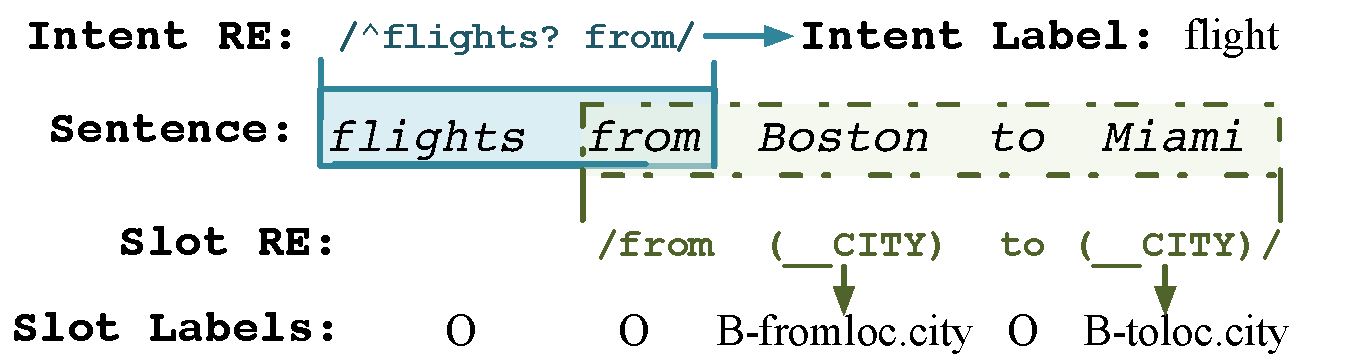
\includegraphics[width=0.49\textwidth]{figure/motivation.pdf}\\
  \vspace{-3mm}
  \caption{A sentence from the ATIS dataset. \REs can be used to detect the intent and label slots.}
  \label{atis_sample}
  \vspace{-3mm}
\end{figure}

\vspace{-1mm}
\subsection{Typesetting}
\vspace{-1mm} In this paper, we use italic for emphasis like \emph{intent detection}, the Courier typeface for abbreviations like
\texttt{RE}, bold italic for the first appearance of a concept like \emph{\textbf{clue words}}, Courier surrounded by / for regular
expressions like {\small \texttt{/list(\;the)?\;\_\_AIRLINE/}}, and underlined italic for words of sentences in our dataset like
\underline{\textit{Boston}}.


\vspace{-1mm}
\subsection{Problem Definition}
\vspace{-1mm}
%While our approach is generally applicable, to have concrete and measurable objectives,
Our work targets two \SLU tasks: \emph{intent detection} and \emph{slot filling}. The former is a sentence classification task where we
learn a function to map an input sentence of $n$ words, $\textbf{x}=[x_{1}, ..., x_{n}]$, to a corresponding \textbf{\emph{intent label}},
$c$. The latter is a sequence labeling task for which we learn a function to take in an input query sentence of $n$ words,
$\textbf{x}=[x_{1}, ..., x_{n}]$, to produce a corresponding labeling sequence, $\textbf{y}=[y_{1}, ..., y_{n}]$, where  $y_i$ is the
\textbf{\emph{slot label}} of the
corresponding word, $x_i$. % in the input query.


%Intent detection is a typical sentence classification task.
%We need to learn a mapping function that maps an input sentence $\textbf{x}$, where $\textbf{x}=[x_{1}, ..., x_{n}]$ is the input sentence with $n$ words, to the corresponding intent $y$.
%% $f: \mathcal{X} \rightarrow \mathcal{Y}$
%% Given a set of training examples $\{(x_i, y_i): i=1,...,N\}$,
%
%On the other side, slot filling is often treated as a sequence labeling task.
%We need to learn a mapping function that maps an input query sentence $\textbf{x}$ to the corresponding label sequence $\textbf{y}$, where $\textbf{y}=[y_{1}, ..., y_{n}]$ is the slot labels of each word.
% Here we also have a set of training examples $\{(\textbf{x}_i, \textbf{y}_i): i=1,...,N\}$, where $\textbf{x}_i=[x_{i1}, ..., x_{in_i}]$ is the input sentence with $n_i$ words, and $\textbf{y}_i=[y_{i1}, ..., y_{in_i}]$ is the slot label of each word.

%For example, Figure\ref{atis_sample} shows a sample sentence in the ATIS dataset. Its intent is \emph{flight}, indicating the user wants
%flight-related information. We also need to identify the \emph{from\_city} and the \emph{to\_city} slots so that the we can return the
%correct information.

%\cparagraph{Example}
Take the sentence in Fig.~\ref{atis_sample} as an example.
%gives an example sentence from the ATIS (Airline Travel Information Systems) dataset~\cite{hemphill1990atis}.
A successful intent detector would suggest the intent of the sentence as \emph{flight}, i.e., querying about flight-related information. A
slot filler, on the other hand, should identify the slots \emph{fromloc.city} and \emph{toloc.city} by labeling \underline{\textit{Boston}}
and \underline{\textit{Miami}}, respectively,
%the sentence
using the begin-inside-outside (\texttt{BIO}) scheme.




\subsection{The Use of Regular Expressions}
\label{re_desc} \vspace{-1mm}

In this work, a \RE defines a mapping from a text \emph{pattern} to several \textbf{\emph{\REtags}} which are  the same as or related to
the \textbf{\emph{target labels}} (i.e., intent and slot labels). A search function takes in a \RE, applies it to all sentences, and
returns any texts that match the pattern. We then assign the \REtag(\texttt{s}) (that are associated with the matching \RE) to either the
matched sentence (for intent detection) or some matched phrases (for slot filling).


% If a \REtag indicates an intent, it would be the same as an intent label.
Specifically, our \REtags for intent detection are the same as the intent labels.
For example,  %when applying the intent \RE
in Fig.~\ref{atis_sample},
% to the example sentence,
we get a \REtag of \emph{flight} that is the same as %corresponds to
 the intent label \emph{flight}.


% an \RE of \texttt{/\textasciicircum
% flights?\:from/} can be associated with an intention label \emph{flight}; and when applying this \RE to the sentence given in
% Figure~\ref{atis_sample} for intention detection, we get a \REtag of \emph{flight}.

For slot filling, we use two different sets of \REs. Given the group functionality of \RE, we can assign \REtags to our interested
\textbf{\emph{\RE groups}} (i.e., the expressions defined inside parentheses). The translation from \REtags to slot labels depends on how
the corresponding \REs are used. (1) When \REs are used at the network module level (Sec.~\ref{interact_with_module}), the corresponding
\REtags are the same as the target slot labels. For instance, the slot \RE in Fig.~\ref{atis_sample} will assign \emph{fromloc.city} to the
first \RE group and \emph{toloc.city} to the second one. Here,  {\small \texttt{\_\_CITY}} is a list of city names, which can be replaced
with a \RE string like \texttt{\small/Boston|Miami|LA|.../}. (2) If \REs are used in the input (Sec.~\ref{fusion_with_input}) and the
output layers (Sec.~\ref{fusion_with_output}) of a \NN, the corresponding \REtag would be different from the target slot labels. In this
context, the two \RE groups in Fig.~\ref{atis_sample} would be simply tagged as \emph{city} to capture the commonality of three related
target slot labels: \emph{fromloc.city}, \emph{toloc.city}, \emph{stoploc.city}. Note that we could use the target slot labels as \REtags
for all the settings. The purpose of abstracting \REtags to a simplified version of the target slot labels here is to show that \REs can
still be useful when their evaluation outcome does not exactly match our learning objective. Further, as shown in Sec.~\ref{re_in_exp},
using simplified \REtags can also make the development of \REs easier in our tasks.
%
%(1)~For the method in Sec.~\ref{interact_with_module}, since we need to annotate clue words for certain slot labels, its \REtags are the
%same as our target slot labels. For example, the slot \RE in Fig.~\ref{atis_sample} will assign \emph{fromloc.city} to the first \RE group
%and \emph{toloc.city} to the second group.
%% \texttt{/(from)\:(\_\_CITY)/} will match the sentence in Figure~\ref{atis_sample}, and assign \emph{fromloc.city} to the second \RE group.
%Here, \emph{\_\_CITY} is a full list of city names, which can be replaced with a string like \texttt{/Boston|Miami|LA|.../}.
%%Note that, an ordinary word list pattern can be written as strings like \texttt{/(\_\_CITY)/} in \RE.
%(2)~For the methods in Sec.~\ref{fusion_with_input} and \ref{fusion_with_output}, the
%\REtag is different from the target slot label.
%For example, the first and second \RE groups in the slot \RE of Fig.~\ref{atis_sample} can be simply tagged as \emph{city},
%% the second \RE group in \texttt{/(from)\:(\_\_CITY)/} will be tagged as \emph{city},
%which is a simplified version of the target slot label, related to three slot labels: \emph{fromloc.city}, \emph{toloc.city}, \emph{stoploc.city}.
%\red{The reason that we use different \REs is to give an example that \REs, with simplified output labels, can also make improvements to
%\NNs.}

% We use another set of \texttt{RE}s for the methods in Sec.~\ref{fusion_with_input} and \ref{fusion_with_output} because using simpler tags can significantly reduce the complexity of the \RE, and therefore making the generation of \RE much easier. For example, we need \texttt{/(from)\:(\_\_CITY)/} to identify \emph{fromloc.city}, but only \texttt{/(\_\_CITY)/} to identify \emph{city}.

%When writing \REs,
Intuitively, complicated \REs can lead to better performance but require more efforts to generate. %, \RE complexity is often an
 Generally, there are two aspects affecting \RE complexity most: the number of \RE groups\footnote{
	When discussing complexity, we consider each semantically independent consecutive word sequence as a \RE group (excluding clauses, such as \texttt{\textbackslash w+}, that can match any word).
	For instance, the \texttt{RE}: {\small \texttt{/how\:long(\:\textbackslash w+)\{1,2\}?\:(it\:take|flight)/}} has two RE groups: {\small \texttt{(how\;long)}} and {\small \texttt{(it\;take|flight)}}.
}
and \emph{or} clauses (i.e., expressions separated by the disjunction operator $|$) in a \RE group. Having a larger number of \RE groups
often leads to better precision but lower coverage on pattern matching, while a larger number of \emph{or} clauses usually gives a higher
coverage but slightly lower precision.


% First, \RE complexity increases with the number of \RE groups. This kind of complexity will lead to better precision but lower coverage. Second, \RE complexity also increases with the number of \emph{or}s (the symbol $|$) in a \RE group. Here a group can be considered as a set of phrases that express the same meaning. Therefore, this kind of complexity usually results in higher coverage and slightly lower precision.
% unless adding ambiguous phrases to the group

% Note that, while the outputs are the intent or slot themselves in the examples above, the \RE output can also be a tag related to, but not the same as, the label that we want to predict.
% We allow this variation because using tags different from the target labels can sometimes make it easier to write an \RE. For example, we need \texttt{/from\:(\_\_CITY)/} to identify \emph{fromloc.city}, but only \texttt{/(\_\_CITY)/} to identify \emph{city}. In this paper, the output of intent patterns is the same as the intent label, and the output of slot patterns used by the method in Section \ref{interact_with_module} is the same as the slot label. However, the slot \RE tag for methods in Section \ref{fusion_with_input} and \ref{fusion_with_output} is the entity part of the slot label (e.g., \emph{city} in \emph{fromloc.city}).
